\documentclass[12pt,letterpaper,twoside]{article}

\newif\ifsolution\solutiontrue   % Include the solutions
%\newif\ifsolution\solutionfalse  % Exclude the solutions

\usepackage{cme213}
\usepackage{xcolor}
\usepackage{float}
\usepackage{graphicx}

\newcommand{\T}[1]{\text{\texttt{#1}}}
\newcommand{\V}[1]{\text{\textit{#1}}}

\begin{document}

{\centering \textbf{Homework 4: CUDA GPU Matrix Operations\\}}
\vspace*{-8pt}\noindent\rule{\linewidth}{1pt}

Goal of the homework is to implement a finite difference solver for the
2-dim heat equation using CUDA GPU programming.

\paragraph{Problem 1: Implement global memory kernel } Idea: parallelize spatial
dimension updates for each time step iteration. One key challenge was to handle
the different border sizes for order inputs of 2, 4 and 8. Kernel logic included
below.

\begin{cpp}
/**
 * Kernel to propagate finite difference grid from the current
 * time point to the next.
 */
template<int order>
__global__
void gpuStencilGlobal(float* next, const float* __restrict__ curr, 
                      int gx, int nx, int ny, float xcfl, float ycfl) {
    
    int borderSize = (int) (order / 2);
    int i = blockIdx.x * blockDim.x + threadIdx.x;
   
    if (i < nx*ny) {
	int x = borderSize + (int) (i / nx);
	int y = borderSize + (i % nx);
        int idx = gx * y + x;   
        next[idx] = Stencil<order>(&curr[idx], gx, xcfl, ycfl);
    
    }
}
\end{cpp}

3D surface plots of temperature on 256x256 grid at iterations 0, 1000 and 
2000 respectively, with 8th order. To do this, I used parameter settings of:
order = 8 and nx = ny = 248. As expected for heat diiffusion, our solution
tends towards a low entropy state of constant temperature.

\begin{figure}[!htbp]
    \centering
    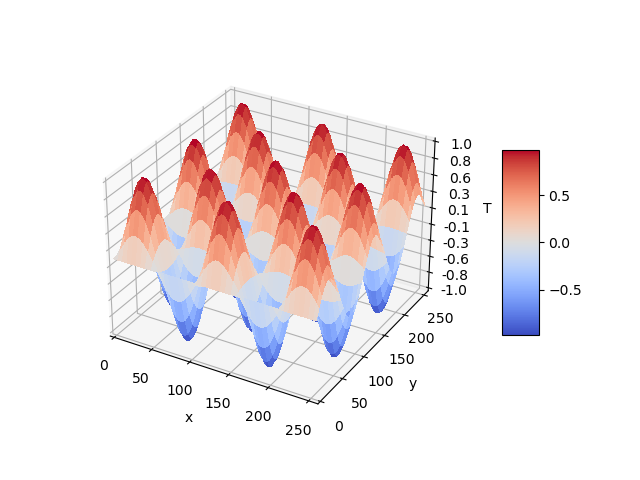
\includegraphics[scale=0.7]{global_0000.png}
    \caption{3D surface plot of temperature at iteration 0}
\end{figure}

\begin{figure}[!htbp]
    \centering
    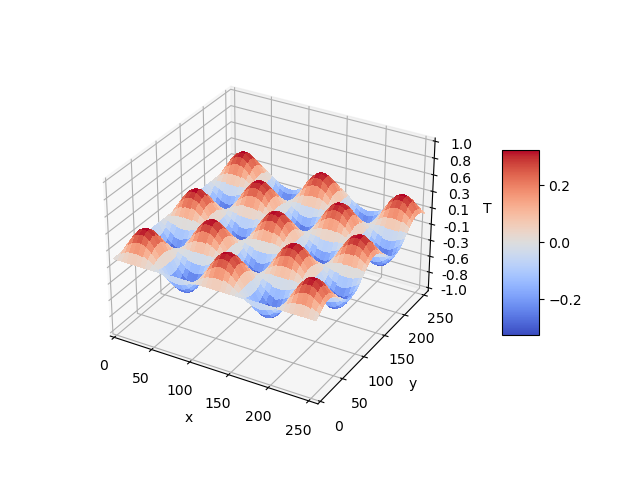
\includegraphics[scale=0.7]{global_1000.png}
    \caption{3D surface plot of temperature at iteration 1000}
\end{figure}

\begin{figure}[!htbp]
    \centering
    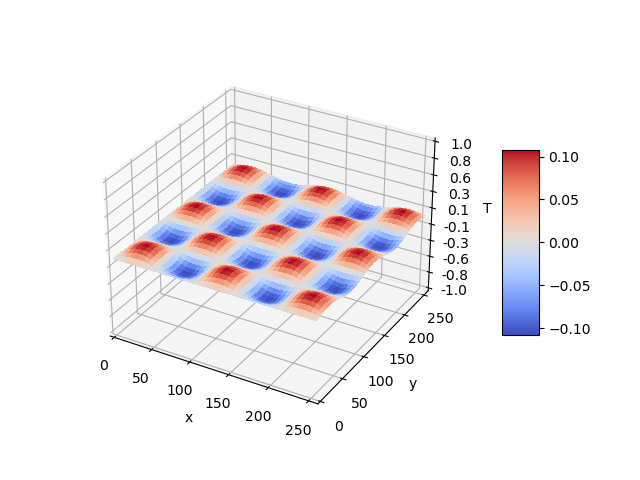
\includegraphics[scale=0.7]{global_2000.png}
    \caption{3D surface plot of temperature at iteration 2000}
\end{figure}

Performance in terms of both time (ms) and bandwidth (Gb/sec) are much 
better already than those observed for CPU computation. Console logs 
included at end of this document.


\paragraph{Problem 2: Implement global memory block kernel } Idea: re-write 
kernel to compute finite difference updates in blocks of size (\texttt{blockDim.y} 
* \texttt{numYPerStep}) * \texttt{blockDim.x}. It should still only use 
global memory.

In order to ensure each thread calculates at most \texttt{numYPerStep} updates, we add 
a for loop inside the kernel (sequential y steps for each thread) and change thread 
block indexing for y dimension to be multiples of \texttt{numYPerStep}.

\begin{cpp}
/**
 * Kernel to propagate finite difference grid from the current
 * time point to the next.
 *
 * This kernel should be optimized to compute finite difference updates
 * in blocks of size (blockDim.y * numYPerStep) * blockDim.x. Each thread
 * should calculate at most numYPerStep updates. It should still only use
 * global memory.
 */
template<int order, int numYPerStep>
__global__
void gpuStencilBlock(float* next, const float* __restrict__ curr, int gx, int nx, int ny,
                    float xcfl, float ycfl) {
    
    int border = (int) (order / 2);
    int i = blockIdx.x * blockDim.x + threadIdx.x;
    int j = (blockIdx.y * blockDim.y + threadIdx.y)*numYPerStep;

    if (i < nx) {
	    int x = i + border;  // x coordinate of matrix
        int niter = min(numYPerStep, ny-j);  // number of updates thread computes
        for (int it = 0; it < niter; it++) {
            int y = j + it + border;
                int idx = gx * y + x;
                next[idx] = Stencil<order>(&curr[idx], gx, xcfl, ycfl);
        }
    }
}
\end{cpp}

Performance in terms of both time (ms) and bandwidth (Gb/sec) improved significantly
compared with \texttt{gpuStencilGlobal}. Console logs included at end of this document.


\paragraph{Problem 3: Plot bandwidth by grid size } Idea: want to understand how the 
different algorithms perform in terms of bandwidth as we increase the scale of the 
problem (grid size).

To do this, we fixed iterations to be 100 and used the following grid sizes: 
256x256; 512x512; 1024x1024; 2048x2048; 4096x4096.

\begin{figure}[!htbp]
    \centering
    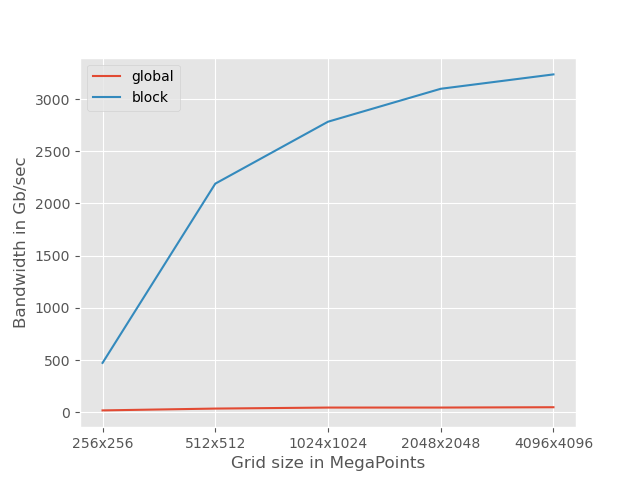
\includegraphics[scale=0.7]{bandwidth_by_alg_ord8.png}
    \caption{Bandwidth vs grid size for different algorithms at order 8}
\end{figure}

Figure 4 illustrates how bandwidth changes with grid size at order 8 for our three 
different algorithms: global, block and shared. As we might expect, bandwidth 
initially increases with grid size (as we increase the number of warps 
simultaneously making requests to global memory), and asymptotically 
approaches a limit that represents our memory bound. Interestingly 
the block algorithm achieves higher bandwidth than shared and 
global algorithms for all larger grid sizes.

\begin{figure}[!htbp]
    \centering
    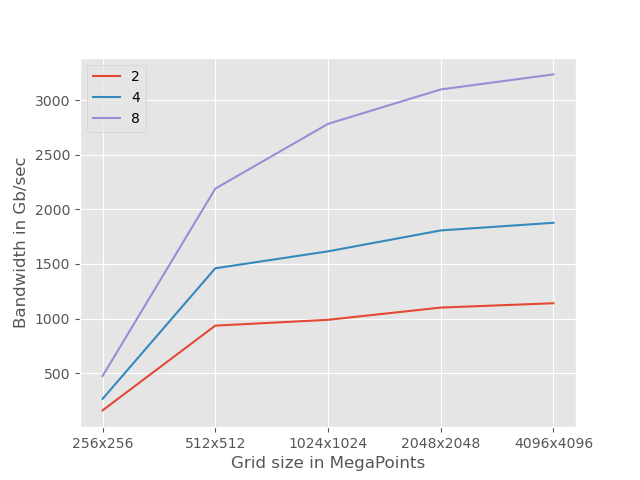
\includegraphics[scale=0.7]{bandwidth_by_order_block.png}
    \caption{Bandwidth vs grid size for block algorithm at orders 2, 4 and 8}
\end{figure}

Figure 5 illustrates how bandwidth changes with grid size for our block algorithm 
as we increase grid size for orders 2, 4 and 8. As expected, bandwidth improves 
as we increase order of our stencil. This is because a higher order stencil will 
be making more coalesced requests to global memory.

\begin{figure}[!htbp]
    \centering
    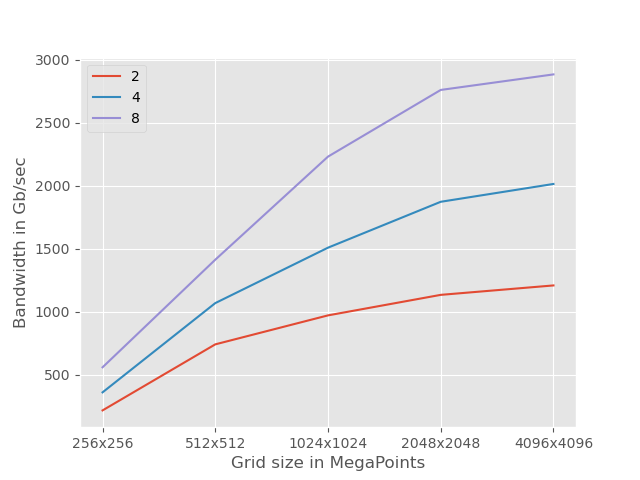
\includegraphics[scale=0.7]{bandwidth_by_order_shared.png}
    \caption{Bandwidth vs grid size for shared algorithm at orders 2, 4 and 8}
\end{figure}

Figure 6 illustrates how bandwidth changes with grid size for our shared memory
algorithm as we increase grid size for orders 2, 4 and 8. Similar to our block 
algorithm, we see bandwidth improves as we increase order of the stencil. This 
is because a higher order stencil will be making more coalesced requests to 
shared memory associated with each thread block.


\paragraph{Problem 4: Explain performance results } For my implementation, the block
kernel for order 8 stencil achieved the best bandwidth (Gb/sec) across all grid sizes.
However, my shared kernel performed comparably on time (ms) and was sometimes faster 
at higher grid sizes, iterations and order.

Bandwidth is the number of memory accesses divided by total execution time. In general, 
as you increase the number of warps requesting memory, you hide the latency of 
the memory pipe.

\begin{itemize}
    \item \textbf{Difference among kernels. } The block kernel outperformed both shared 
    and global kernels (figure 4). While this was expected for the global kernel given our block 
    implementation should result in more cache hits, the shared memory performance was 
    surprising. This may be due to bank conflicts or calibration of thread block 
    dimensions vs \texttt{numYPerStep}.

    \item \textbf{Difference from varying order. } As you increase stencil order, 
    you improve the memory request pattern of each warp to be more coalesced.
    This hides latency and improves bandwidth (figure 5).

    \item \textbf{Difference from varying problem size. } As you increase grid size, 
    you increase the number of warps requesting memory in parallel, which hides 
    latency and improves our bandwidth. This improvement will asymptotically 
    approach the memory bound (figures 4, 5 and 6).

\end{itemize}


\paragraph{Problem 5: Implement shared memory block kernel } Idea: copy across current 
array values into shared memory to reduce access requests to global memory and make use 
of higher shared memory access speeds (lower latency because closer to each processor 
core). We do this at the thread block level since we are guaranteed warps within a 
thread block share the same SM and therefore shared memory. 

One key challenge was that each thread block needs to be able to access more values from 
the current array than it updates (based on stencil order). This means our shared memory 
blocks are necessarily overlapping to ensure we update the whole array. We enforce this 
"overlapping" thread block behaviour through our mapping of thread id to our current 
array index. Kernel logic included below.

\begin{cpp}
/**
* Kernel to propagate finite difference grid from the current
* time point to the next.
*
* This kernel should be optimized to compute finite difference updates
* in blocks of size side * side using shared memory.
*/
template<int side, int order>
__global__
void gpuStencilShared(float* next, const float* __restrict__ curr, int gx, int gy,
               float xcfl, float ycfl) {
    
    // map thread to global position
    int border = order / 2;
    int numY = side / blockDim.y;
    int sub_square_side = side - order;
    int i = blockIdx.x*sub_square_side + threadIdx.x;
    int j = blockIdx.y*sub_square_side + threadIdx.y*numY;
    
    // load mesh grid into shared memory
    __shared__ float shared[side][side];
    if (i < gx) 
    {
        int niter = min(numY, gy-j);  // number of updates thread computes 
	for (int it = 0; it < niter; it++) {
	    if ((j+it) < gy) {
	        shared[threadIdx.y*numY+it][threadIdx.x] = curr[gx*(j+it)+i];
	    }
	}
    }
    __syncthreads(); 

    // apply stencil inside domain
    if (i < (gx-border) &&
	threadIdx.x >= border && 
	threadIdx.x < (side-border)) 
    {
        int niter = min(numY, gy-j);  // number of updates thread computes 
        for (int it = 0; it < niter; it++) {
            if ((j+it) < (gy-border) &&
                (threadIdx.y*numY+it) >= border &&
                    (threadIdx.y*numY+it) < (side-border)) 
            {
                next[gx*(j+it)+i] = Stencil<order>(
                    &shared[threadIdx.y*numY+it][threadIdx.x], 
                    side, 
                    xcfl, 
                    ycfl);
            }
        }
    }
} 
\end{cpp}

\pagebreak
Console logs from executing our kernels for grid size 1024x1024
at order 8 for 400 iterations.

\begin{verbatim}
Output from main
----------------
Order: 8, 4096x4096, 100 iterations
                        time (ms)     GBytes/sec
            CPU           2661.73        45.3824
            Global        50.2889        2402.04
            Block         37.3118        3237.48
            Shared        41.8833        2884.11

                            L2Ref           LInf          L2Err
            Global       0.447065              0              0
            Block        0.447065              0              0
            Shared       0.447065              0              0
\end{verbatim}


Submission information logs.
\begin{verbatim}
jelc@cardinal2:~$ /afs/ir.stanford.edu/class/cme213/script/submit.py hw4 private/cme213-jelc53/hw4/
Submission for assignment 'hw4' as user 'jelc'
Attempt 1/10
Time stamp: 2022-05-19 00:20
List of files being copied:
    private/cme213-jelc53/hw4/gpuStencil.cu	 [12599 bytes]

Your files were copied successfully.
Directory where files were copied: /afs/ir.stanford.edu/class/cme213/submissions/hw4/jelc/1
List of files in this directory:
    gpuStencil.cu	 [12599 bytes]
    metadata	 [137 bytes]

This completes the submission process. Thank you!
    

jelc@cardinal2:~$ ls /afs/ir.stanford.edu/class/cme213/submissions/hw4/jelc/1
gpuStencil.cu  metadata

\end{verbatim}

\end{document}
